\chapter{Implementation, Analysis and Results}
{\color{red} 
	Investigation of constraints impact in time windows was performed by analysing two different types of association networks; the networks with fixed step size nodes and the networks with fixed bucket size nodes.
	
	Those two different types of networks were applied in all ten time-window, and average modularity metric plots were generated. 
}

\section{Real-life Events}
The steel manufacturing events were analysed in six different dimensions: Production Line, Production Constraint, Production Feature, Time, Network Resolution and Null Model.

For the first dimension, distinguished data sets were considered among four different production lines: Continuous Casting Machine (CCM), Compact Strip Production (CSP), Continuous Galvanizing Line (CGL), and Pickling Line \& Tandem Cold Mill (PLTCM). In principle, CCM and CSP production lines have similar functionalities; however, they were kept separated in the analysis pipeline since their labels are different in the database.
{\color{red}
	Show the production lines with a table listing names and explanations of each production line. Refer to that table when I interpret my findings.
}

Two fundamentally different constraints acting on the manufacturing process: technology-driven constraints and load-driven constraints, were shaped hypothetically and defined as two distinguished network approaches: fixed step-sized and fixed bucket-sized networks. Those attempts are in the second dimension of the analysis. 

As the third dimension, slabs' width and thickness features were picked to investigate different production constraints that play a role in the machines for those features. 

Time is the fourth dimension and considered to check constraints impact on the historically ordered production events. The data set was treated in both discrete-time windows and increasing-time windows to study the behaviour of changing fixed step size and fixed bucket size. 

Generated networks were diversified in two different resolutions by changing the node amount in the fifth dimension. As a concept of characterising, modularity was calculated for the networks. The aim is to keep the networks with a similar number of nodes in both network approaches (fixed step size and fixed bucket size) so that the modularity quantification would be meaningful to compare. 

As the last dimension, two types of null models: shuffling the links in degree conservation and shuffling them based on the communities, were considered to check the randomness of the networks. Obtained Z-scores can vary based on the generated null model via that specific randomisation method.

The data sets were partitioned into two halves, and analysis steps were applied for the first half, second half, and the complete data set. At the top of bar chart sets, modularity values were presented for the original network and a single randomised network. Z-scores belong to different null models for $1000$ randomised networks were given in the bottom part of the bar chart set, indicated with a colourless line finish. For each of the z-scores, error bars were included by removing and putting back 10\% of the data several times (a check for the robustness of the statistical signals). The coloured bar border indicates the mean value, and the T-shaped symbol represents the standard deviation of the error bars.

Constraints are clearly different for the different production lines, emphasising the shift from width to thickness when changing to another production line. 

\subsection*{Data Collection and Cleaning}
\addcontentsline{toc}{subsection}{Data Collection and Cleaning}%

The SQL queries were generated to find and pull the production orders in a range of $2$ to $3$ years belong to CCM, CSP, CGL, and PLTCM from the SMS database. The SQL queries are given in the Supplementary Materials (\ref{figure-supplements-CCM_CSP-SQL}, \ref{figure-supplements-CGL-SQL}, and \ref{figure-supplements-PLTCM-SQL}). 

At the beginning of the data cleaning process, the raw data was handled considering the string-type data values conversion into floating-point numbers, modifying inconsistent punctuation marks between digits into one typical style, and converting null values into the integer value $0$. 

After going over minor revision steps, we introduce some preconditions below to consider usable parts and fill the gaps in the data sets.
\begin{itemize}
	\item The steel material density was considered between $6.5 x 10^{-6}$ $kg/mm^{3}$ and $8.5 x 10^{-6}$ $kg/mm^{3}$. The production orders with density values out of that range were discarded from consideration.
	\item The production feature, length values were taken into account with millimetre (mm) units in the metric system.
	\item Production capacity limit ranges were identified for the production features, width, thickness, and weight as $800$--$2000$ mm, $40$--$90$ mm, and $2669$--$26690$ kg.
\end{itemize}

Considering the preconditions mentioned above and $density = mass/volume$ equality, $0$ values were replaced with the calculated values in every production order with a maximum of one unknown value from the features; width, thickness, weight, and length. Production orders (the so-called events) with two missing values were compared with consecutive events, and missing terms were filled based on the consistency among the sequence events. Sequences with less than $50$ events were removed from the data sets considering those short sequences might be generated for some test processes. At the final stage, obtained data set lengths are given below.
\begin{itemize}
	\item CCM data set: $347,418$ events.
	\item CSP data set: $205,496$ events.
	\item CGL data set: $31,230$ events.
	\item PLTCM data set: $64,026$ events.
\end{itemize}

\subsection*{Analysis and Results}
\addcontentsline{toc}{subsection}{Analysis and Results}%

Time Windows Generation by Data Partitioning:

the dataset with length 396096 was partitioned into ten time-window starting from the beginning of the data. In each step, it's increased by 39610 rows more or less (increasing windows). The exact increase step dimension was specified by the last order of the corresponding sequence. For my dataset, exact time window lengths are 39871, 79567, 118358, 158421, 198041, 237352, 277147, 316411, 356385, 396096. Almost always the same statistics for every window. Abnormal increase modularity increase towards the end due to increasing window size. If there is a shift in how the data behaves, I will almost not see it because it is mast by the other data present in my analysis. The modularity curves seem to drift a little bit upwards. There is a trend of going up no matter how it behaves in the middle. My reason was to do this to check the load effect.

Partitioning was repeated with discrete-time windows (sliding windows). Shifting window within equal windows size. To see the results of the same analysis in each discrete time window. Whether the rules I discovered from the first dataset (1st time-window) and the second dataset (2nd time-window) are really fundamentally different or rather the same.

 \begin{figure}[!ht]
	\begin{center}
		\makebox[\textwidth]{
			\centering
			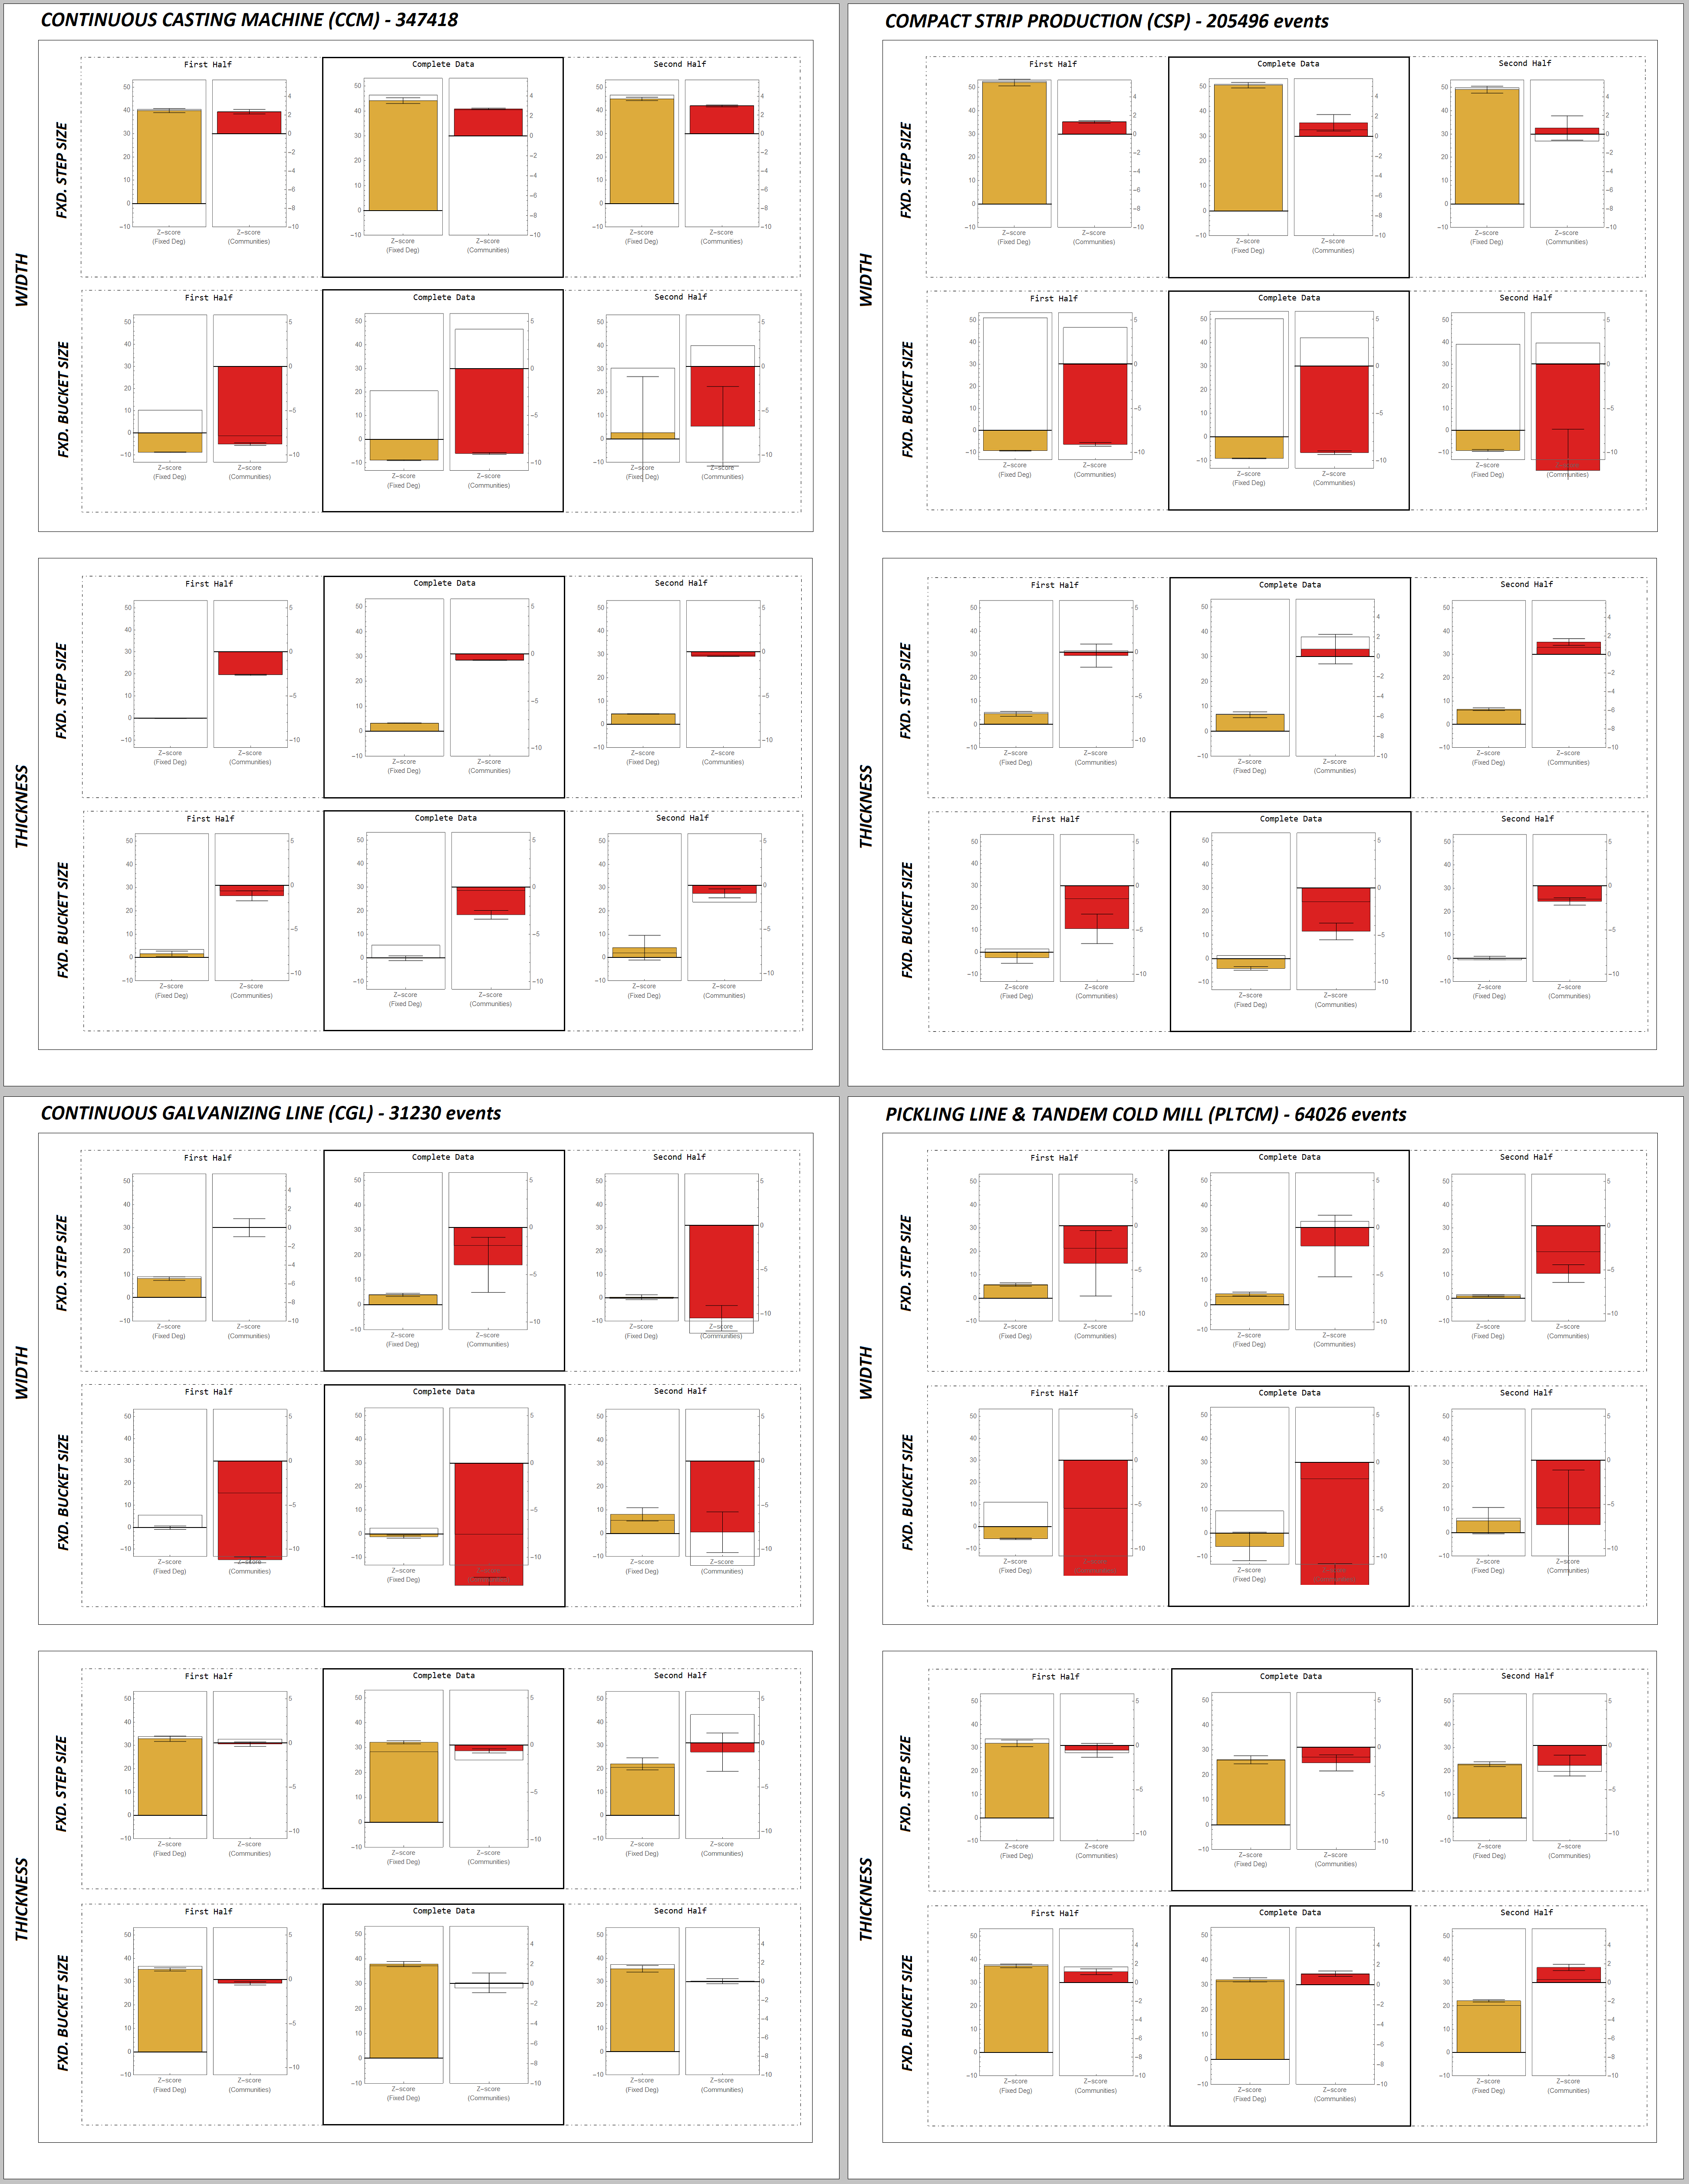
\includegraphics[width=1.05\linewidth]{../images/results-real_life_events_analysis-results.png}}
		\caption{CCM, CSP, PLTCM, CGL \aa{} Z-scores.}
		\label{figure-real-life-events-analysis-results}
	\end{center}
\end{figure}



{\color{red}
	%	24.03.21
	Regarding behaviour on networks with changing FSS and FBS amounts, the first column plots show a calibration curve with graph node numbers corresponding to changing FSS and FBS. The FBS paradigm leads to higher modularity for the weight feature than the FSS paradigm, no matter which bucket/step size we pick. This result becomes the opposite when it comes to length and width. For thickness, there is no clear result to say as the others have. They are actually sometimes on the same level. The fact that modularity tends to be higher in one paradigm and lower in the other which is an interesting thing.
	
	Investigating constraints impact among the data in a time-resolved fashion confirms my previous investigation of the data with increasing time windows.
	
	Our hypothesis at the moment is that the physical constraints are rather about step sizes than being about bucket sizes because step size graphs are less random.
	
	In my previous project, the fixed step size graphs had high modularity. That means that the actual quantity I discretise creates the constraints, while in the case of fixed bucket size, it would be the volume of orders that makes my constraints. That summarises our hypothesis. 
	
	%	What I would get = On the width level, we have a reasonably constant behaviour over time, and it confirms what I see on the total dataset, a big difference in modularity between the two network approaches. For the FBS approach, there might be a transition. The fixed bucket size becomes very modular in the end.
	
	For thickness, it's less apparent because the modularity is at the same level for both FSS and FBS, but the increase in modularity for FBS is reasonably dramatic. It goes from 0.3 to 0.6 while the other remains at 0.3 and fluctuates. In the last two time windows in FBS, the process is dominated by something else. It is evident that something changed of the constraints involved really takes place.
	
	current situation
	The Modularity (Single Random Graph) and Z-score plots, dashed curves are provided for the Fixed Degrees Null Model and unbroken curves are provided for Modularity Null Model.
	Network node numbers were kept equal for the same time windows in different network approaches but not in the consecutive time windows in the same network approaches.
	Other than the below-given networks, including fewer nodes than 15 in some cases, all networks have varying node numbers between 25-90.
	\begin{itemize}
		\item CSP Thickness Network with narrow node binning
		\item CSP Thickness Network with large node binning
		\item CCM Thickness Networks with narrow and large node binning
	\end{itemize}
	
	before treating time windows, having the modularity as function of bucket size and as function of step size. At this stage, choosing suitable step and bucket sizes and accordingly repeat all progress mentioned above. The aim is to obtain big amount of nodes as possible as we can and keeping that amount of nodes the same in both graph structures (fixed step size and fixed bucket size). The difference between modularity values at highest graph nodes amount in fixed bucket and fixed step sized graphs shows which network structure is more effective on generating clear communities. In other words, modularity values is more meaningful when the node number is high.
	
	Results are not stable, which is a bit expected with these complicated data structures. This is why we do the sensitivity analysis on top of that: varying the resolution, doing things with slightly different methods (different null models) over and over again.
	
	Is the dashed curve of FSS higher than the dashed curve of FBS? That's a type of information we should extract from those plots/bar charts.
	I am trying to figure out whether the step from FSS to FBS drastically changes the modularity. I am wondering whether we can condense this further to make this information is more accessible.
	Z-scores plot are more honest compared to modularity plot because it takes out any effect that comes from different link densities.
	
	In some sense, we try to do the data as simpler as they are, by trying to pretend that they are more homogeneous than they are. We pretend that the data is statistically reliable and not distorted and most of all that this temple of the modular network really fits. All of these assumptions are slightly wrong, what we see here is the consequence of that. We need to try to make the statistical assumptions about the data that are not necessarily fulfilled and these assumptions can lead to things sometimes looking statistically significant even though they are not. And those statistical assumptions are most of the time that the data are not very distorted but somehow reliably distributed. And top of that, modularity as a fairly simple concept of characterising networks, is a meaningful concept here. We should say that these are all assumptions.
}
\clearpage

\section{Simulation Events}
\subsection*{Analysis and Results}
\addcontentsline{toc}{subsection}{Analysis and Results}%

{\color{red} 
	
	Briefly explain \emph{in silico analyses} attempts /numerical experiments from the generated data.
	
	Plots in Part-1 of the file belong to association networks of four different synthetically created sequence data sets, and each represented in various colors: green, blue, orange, and red. Part-1 data sets were derived with fixed reaction bounds but with varying coefficients of objective functions. Part-2 also presents plots for four different synthetically created sequence data sets with fixed objective function coefficients but with variable reaction bounds.
	
	Each data set has a length of 10,000 events shared equally in 200 sequences. Randomly picked subsets of fluxes were kept the same within the sequences but having varying coefficients of objective functions.
	
	
	
	Limitation on resources were performed in two different ways; first, restriction on upper \& lower bounds and second, deletion of fluxes.
	
	The fluxes used in the intermediate reactions were given the range of bounds as $(-500, 500)$ since it is not possible to define infinity values in the optimisation algorithm. Randomly chosen $105$ fluxes out of $1008$ were matched with $(-5, 5)$ as the first step. And $105$ was doubled ($212$) and then quadrupled ($425$). An important detail is all of the three sets of choices were done randomly, they are not added on top of already selected $105$. In every further step, the same three sets of fluxes were used in the computations as restricted bounds.
	
	Deletion goes in the line: $0, 50, 100, 150, 200, 250, 300, 350, 400, 450$. As explained previously, deletion was done by assigning $(0, 0)$ bounds to the fluxes. On the last step, almost half of the total fluxes ($1008$) were erased.
	
	In an ideal scenario, we would find that association networks derived from the generated data, in the one case; produce high modularity for FBS and in the other case produce high modularity for FSS. Because then we have linked these two data processing schemes to different forms/to different categories of constraints.
	
	We see here that when I vary one constraint about the richness curve plots, I go from a factory that produces anything at random to a more specific factory in their production plans. The modularity at FBS increases, modularity at FSS does not increase. From left to right, I increase the constraint that the production plan (or portfolio of the factory) impose on the whole production process. The production portfolio is grouped into speciality products on the right end. Increase in modularity is only true for the green and orange curves which means that this effects of the changing of portfolio only takes place in addition I impose a certain constraints on the material flow (FBS). I enforce the production plans. In some sense, with the coefficients of obj. function being symmetric around zero, I allow them also to near zero. I allow for the case this product doesn't take place. The red and the blue curves are less interesting, they are rather serving as an orientation. We wouldn't expect them to be severely affected by changes in the richness of the objective function because the terms are cancelled out. So the interesting curves are the green and orange one that we can argue for it. We don't expect a strong impact of the richness of the objective functions for these cases (red and blue), and that's indeed what I numerically observed. So it makes sense to have these curves, but the interesting curves are the green and the orange ones.
	Blue curve z-score is very hard to compute, we should not trust it that much, also its z-score curve is lower compared to red z-score curve. 
}

 \begin{figure}[!ht]
	\begin{center}
		\makebox[\textwidth]{
			\centering
			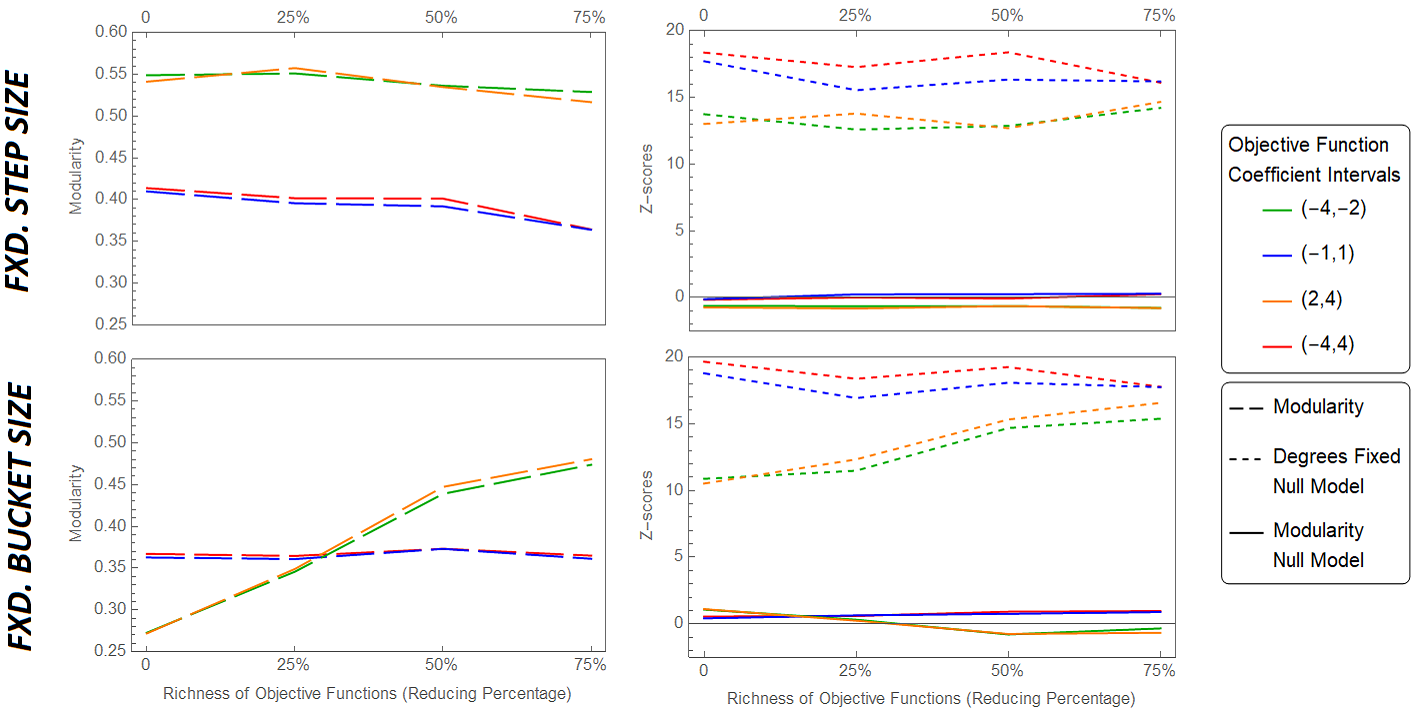
\includegraphics[width=1.03\linewidth]{../images/results-simulation-results.png}}
		\caption{Simulation Analysis Curve Plot Results: Modularity Values and Z-scores.}
		\label{figure-FBA-results}
	\end{center}
\end{figure}

%\begin{equation} %\tag{8}
%	(O.V)_{1}= (o_{1,1}v_{1} + o_{1,2}v_{2} + \dots + o_{1,r}v_{r})
%\end{equation}

%\begin{equation} %\tag{8}
%	(O.V)_{2}= (o_{2,1}v_{1} + o_{2,2}v_{2} + \dots + o_{2,r}v_{r})
%\end{equation}

%\begin{equation} 	
%	(O.V)_{50}= (o_{50,1}v_{1} + o_{50,2}v_{2} + \dots + o_{50,r}v_{r})
%\end{equation}

%\begin{equation} 	
%	(O.V)_{51}= (o_{1,1}v_{1} + o_{1,2}v_{2} + \dots + o_{1,r}v_{r})
%\end{equation}

%\begin{equation} 	
%	(O.V)_{100}= (o_{50,1}v_{1} + o_{50,2}v_{2} + \dots + o_{50,r}v_{r})
%\end{equation}

%\begin{equation} 	
%	(O.V)_{10000}= (o_{50,1}v_{1} + o_{50,2}v_{2} + \dots + o_{50,r}v_{r})
%\end{equation}

%\begin{table}[hb!]
%	\centering
%	\begin{tabular}{|cccccc|l}
%		\cline{1-6}
%		\makecell{Event\\ID} && \makecell{Bio\\Mass} 	&& \makecell{Seq.\\ID} &  \\ \cline{1-6}
%		1 	      && $m_{1}$  	&& 1 		   	&  \\
%		2 		  && $m_{2}$	&& 1 		   	&  \\
%		3 	      && $m_{3}$	&& 2 		    &  \\
%		\vdots	  && \vdots && \vdots 	    &  \\
%		n 		  && $m_{n}$	&& k 		    &  \\ \cline{1-6}
%	\end{tabular}
%	\caption{Arbitrarily Created Data Set $D$.}
%	\label{Tab:D-dataset}
%\end{table}